\documentclass[11pt,a4paper]{article}
\usepackage[hyperref]{acl2018}
\usepackage{times}
\usepackage{latexsym}

\usepackage[letterpaper]{geometry}
%\usepackage{amta2016}
\usepackage{url}
\usepackage{natbib}
\usepackage{layout}

\usepackage{algorithm}% http://ctan.org/pkg/algorithms
\usepackage{algpseudocode}% http://ctan.org/pkg/algorithmicx

\usepackage{graphicx}
\usepackage{amsmath}
\DeclareMathOperator*{\argmax}{argmax}

\newcommand{\confname}{AMTA 2016}
\newcommand{\website}{\protect\url{http://www.amtaweb.org/}}
\newcommand{\contactname}{research track co-chair Lane Schwartz}
\newcommand{\contactemail}{lanes@illinois.edu} 
\newcommand{\conffilename}{amta2016}
\newcommand{\downloadsite}{\protect\url{http://www.amtaweb.org/}}
\newcommand{\paperlength}{$12$ (twelve)}
\newcommand{\shortpaperlength}{$6$ (six)}

%% do not add any other page- or text-size instruction here

\parskip=0.00in

\begin{document}

% \mtsummitHeader{x}{x}{xxx-xxx}{2016}{45-character paper description goes here}{Author(s) initials and last name go here}
\title{\bf Faster Neural Machine Translation Inference}  

\author{\name{\bf Hieu Hoang} \hfill  \addr{hieu@hoang.co.uk}\\ 
        \addr{}
\AND
       \name{\bf Tomasz Dwojak} \hfill \addr{???}\\
        \addr{Adam Mickiewicz University}
\AND
       \name{\bf Kenneth Heafield} \hfill \addr{???}\\
       %\name{\bf Kenneth Heafield} \hfill \addr{kheafiel@inf.ed.ac.uk}\\
        \addr{University of Edinburgh, Scotland}
}

\maketitle
\pagestyle{empty}

\begin{abstract}

We present two optimizations in areas where typical NMT models differ significantly from other deep-learning models. Firstly, we optimize the output layer which takes a significant amount of time for NMT models due to the large number of output classes, corresponding to the output vocabulary. Secondly, we present a novel batching algorithm which takes into account the differing output sentence lengths which leads to inefficiencies in current batch algorithms. Together, we increase inference speed by up to 57\% on modern GPUs without affecting model quality.

\end{abstract}

\section{Introduction}
\label{sec:Introduction}

The number of classes in NMT models is typically in the tens or hundreds of thousands, for example, ~\citet{sennrich-haddow-birch:2016:P16-12} experimented with target vocabulary sizes of 60,000 and 90,000 sub-word units. This makes the output layer of NMT models computationally expensive. Figure~\ref{fig:pie-time-opensubtitles} shows the breakdown of amount of time during translation our NMT system; 73\% of the time is involved in the output layer or beam search. Our first proposal will explicitly target this computation.
\begin{figure}[h]
\centering
\begin{tabular}{cc}
{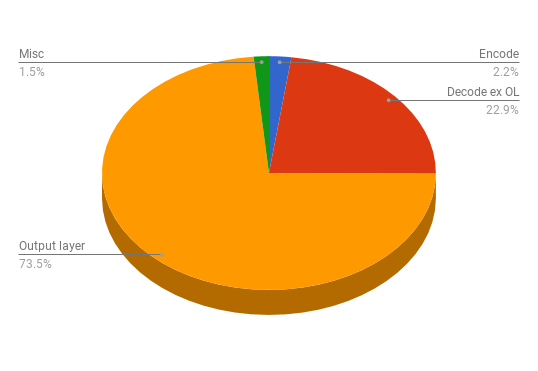
\includegraphics[scale=0.3]{pie-time-opensubtitles.png}} 
\end{tabular}
\caption{Proportion of time spent during translation}
\label{fig:pie-time-opensubtitles}
\end{figure} 

Secondly, the use of mini-batching is critical for fast model inference. However, mini-batching does not take into account variable sentence lengths which decrease the actual number of input or output sentences that are processed in parallel, negating the benefit of mini-batching. This can be partially reduced in the encoding with \emph{maxi-batching}, i.e. pre-sorting sentences by length before creating mini-batches with similar length source sentences. However, maxi-batching can introduce unacceptable delays in response time as inputs are not processed in the order they came, a particular concern for online applications. 

Even with maxi-batching, target sentence lengths will still differ even for similar length inputs. Figure~\ref{fig:batch-size} shows the actual batch size during decoding with a maximum batch size of 128; the batch was full in only 42\% of decoding iterations. We will propose an alternative batching algorithm to increase the actual batch size during decoding without the problems associated with mini-batching and maxi-batching.

\begin{figure}[h]
\centering
\begin{tabular}{cc}
{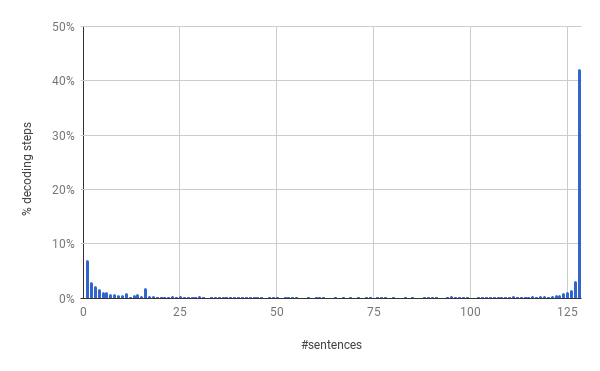
\includegraphics[scale=0.3]{batch-size.png}} 
\end{tabular}
\caption{Actual batch size during decoding}
\label{fig:batch-size}
\end{figure} 

% \section{Prior Work}
% 
% Deep-learning models has been successfully used on many machine learning task in recent years in areas as diverse as computer vision and natural language processing. This success have been followed by the rush to put these model into production. The computational resources required in order to run these models has been challenging but, fortunately, there has been a lot work to meet this challenge.
% 
% Hardware accelerators such as GPUs are very popular but other specialized hardware such as custom processors~\citep{DBLP:journals/corr/JouppiYPPABBBBB17} and FPGA~\citep{DBLP:journals/corr/LaceyTA16} have been used. Hardware-supported reduced precision is also an ideal way to speed up model inference~\citep{DBLP:journals/corr/abs-1710-03740}.
% 
% Simpler, faster models have been created that are as good, or almost as good, as more slower, more complex models~\citep{DBLP:journals/corr/BahdanauCB14}. Research have also gone into smaller, faster models that can approximate slower, bigger models~\citep{DBLP:conf/emnlp/KimR16}. Some models have been justified as more suited for the parallel architecture of GPUs~\cite{DBLP:journals/corr/VaswaniSPUJGKP17}~\cite{gehring2017convs2s}.
% 
% The speed of the softmax layer when used with large vocabularies have been looked at in~\citet{DBLP:journals/corr/GraveJCGJ16} but there have been many other attempts at faster softmax, for example~\citet{DBLP:journals/corr/abs-1301-3781}, ~\citet{Zoph-2016}.
% 
% There has been surprisingly little work on batching algorithms, considering its critical importance for efficient deep-learning training and inference. ~\citet{Neubig-autobatching} describe an novel batching algorithm, however, its aim is to alleviate the burden on developers of batching models rather than faster batching.
% 
% Our paper follows most closely on from ~\citet{DBLP:conf/emnlp/Devlin17} which achieved faster NMT inference mainly by novel implementation of an existing model. However, we differ by focusing on GPU implementation, specifically the output layer, and the batching algorithm which was not touched on by the previous work. Our model is based on that of ~\citet{D14-1179} and ~\citet{sennrich-haddow-birch:2016:P16-12} but our work is applicable to other models and applications. % rather than CPUs as pursued by ~\cite{DBLP:conf/emnlp/Devlin17}.


\section{Proposal}
\label{sec:Proposal}

\subsection{Softmax and Beam Search Fusion}

The output layer of most deep learning models consist of the following steps
\begin{enumerate}
   \item \vspace{-3 mm} multiplication of the weight matrix with the input vector $p = w x$
   \item \vspace{-3 mm} addition of a bias term to the resulting scores $p = p + b$
   \item \vspace{-3 mm} applying the activation function, most commonly softmax $ p_i = \exp(p_i) / \sum \exp(p_i) $
   \item \vspace{-3 mm} a beam search for the best (or n-best) output classes $\argmax_i p_i$
\end{enumerate}

We focus on the last three steps, the outline for which are shown in Algorithm~\ref{algo:original-softmax-beamsearch}. For brevity, we show the algorithm for 1-best, a beam search of the n-bests is a simple extension of this.

As can be seen, the matrix p is iterated over five times - once to add the bias, three times to calculate the softmax, and once to search for the best classes. We propose fusing the three functions into one kernel, a popular optimization technique~\citep{Guevara2009EnablingTP}, making use of the following observations.

Firstly, softmax and $\exp$ are monotonic functions, therefore, we can move the search for the best class from FIND-BEST to SOFTMAX, at the start of the kernel.

\begin{algorithm}
\begin{algorithmic}
\small

\Procedure{AddBias}{vector $p$, bias vector $b$}
\ForAll{$p_i$ in $p$}
  \State $p_i \gets p_i + b_i$
\EndFor 
\EndProcedure

\State

\Procedure{Softmax}{vector $p$}

\Comment{calculate max for softmax stability}
\State $max \gets - \infty$ 
\ForAll{$p_i$ in $p$}
  \If{$p_i > max$}
    \State $max \gets p_i$
  \EndIf
\EndFor

\Comment{calculate denominator} 
\State $sum \gets 0$ 
\ForAll{$p_i$ in $p$}
  \State $sum \gets sum + \exp(p_i - max)$
\EndFor

\Comment{calculate softmax}
\ForAll{$p_i$ in $p$}
  \State $p_i \gets \frac{\exp(p_i - max)}{sum} $
\EndFor 

\EndProcedure

\State

\Procedure{Find-Best}{vector $p$}

\State $max \gets - \infty$ 
\ForAll{$p_i$ in $p$}
  \If{$p_i > max$}
    \State $max \gets p_i$
    \State $best \gets i$
  \EndIf
\EndFor 

\Return $max$, $best$

\EndProcedure

\end{algorithmic}
\caption{Original softmax and beam Search Algorithm}
\label{algo:original-softmax-beamsearch}
\end{algorithm}

Secondly, we are only interested in the probabilities of the best classes. Since they are now known at the start of the kernel, we compute softmax only for those classes. The outline of the our kernel is shown in Algorithm~\ref{algo:Fused Kernel}.

\begin{algorithm}
\begin{algorithmic}
\small

\Procedure{Fused-Kernel}{vector $p$, bias vector $b$}

\Comment{add bias, calculate $max$ \& $argmax$}

\State $max \gets - \infty$ 
\ForAll{$p_i$ in $p$}
  \If{$p_i + b_i > max$}
    \State $max \gets p_i + b_i$
    \State $best \gets i$
  \EndIf
\EndFor

\Comment{calculate denominator}

\State $sum \gets 0$ 
\ForAll{$p_i$ in $p$}
  \If{$p_i > max$}
    \State $sum \gets sum + \exp(p_i - max)$
  \EndIf
\EndFor

\Return $\frac{1}{sum}$, $best$ 

\EndProcedure
\end{algorithmic}

\caption{Fused softmax and beam search}
\label{algo:Fused Kernel}
\end{algorithm}

In fact, we are usually only interested in the best class during inference, not the probability. Since we now compute the best class before the softmax, we can skip softmax altogether. This is only possible for beam size 1; the comparison between softmax probabilities is required for larger beam sizes as the denominators are different for different hypotheses.

\subsection{Top-up Batching}

The standard mini-batching algorithm encode the sentences for a batch, followed by decoding the batch. Decoding stop only once all sentences in the batch are completed.

\begin{algorithm}
\begin{algorithmic}
\small

\Procedure{Encode}{}
\While{more input} 
  \State Create encoding batch $b$
  \State Encode($b$)
  \State Add $b$ to queue $q$
\EndWhile 

\EndProcedure

\end{algorithmic}
\caption{Encoding for top-up batching}
\label{algo:Encoding for top-up batching}
\end{algorithm}

Our proposal focuses on decoding as this is the more compute-intensive task, encoding and decoding asynchronously. The encoding step, Algorithm~\ref{algo:Encoding for top-up batching}, is similar to that in mini-batching except that the results are added to a queue.

The decoding continuously process the same batch, adding new sentences as old sentences completes, Algorithm~\ref{algo:Decoding for top-up batching}.

\begin{algorithm}
\begin{algorithmic}
\small

\Procedure{Decode}{}

\State create batch $b$ from queue $q$
\While{$b$ is not empty}
  \State Decode($b$)
  \ForAll{sentence $s$ in $b$}
    \If{trans($s$) is complete}
      \State Replace $s$ with $s'$ from $q$
    \EndIf
  \EndFor
\EndWhile

\EndProcedure

\end{algorithmic}
\caption{Decoding for top-up batching}
\label{algo:Decoding for top-up batching}
\end{algorithm}


\section{Experimental Setup}
\label{sec:Experimental Setup}

We train a sequence-to-sequence, encoder-decoder NMT system similar to that described in ~\citet{sennrich-haddow-birch:2016:P16-12}. This uses recurrent neural networks with gated recurrent units. The input and output vocabulary size are both set to 85,000 sub-words using byte-pair encoding (BPE), the hidden layer dimensions is 512. %We used the Marian toolkit to train our models.

For inference, we used and extend Amun~\citep{junczys2016neural}. We used a beam size of 5, mini-batch of 128 sentences and maxi-batch 1280, unless otherwise stated.

The hardware used in all experiments was an Nvidia GTX 1060 GPU on a host containing 8 Intel hypercores running at 2.8Ghz, 16GB RAM and SSD hard drive.

The German-English version of the Europarl corpus~\citep{Koehn:2005:MTS} was used to train the model, our test set consisted of the first 50,000 sentences of the Open-Subtitles corpus~\citep{TIEDEMANN12.463}.

\section{Results}
\label{sec:Results}

\subsection{Softmax and Beam Search Fusion}

Fusing the last 3 steps led to a substantial reduction in the time taken, especially for beam size of 1 where the softmax probability does not actually have to calculated, Table~\ref{tab:fused-breakdown-opensubtitles}. This led to an overall increase in translation speed of up to 41\%, Figure~\ref{fig:beam-opensubtitles}. 

\begin{table}
\begin{center}
\small
\begin{tabular}{|l|r|r|} \hline
		& Baseline	& Fused \\ \hline
\multicolumn{3}{|c|}{\emph{Beam size 1}}	\\ \hline	
Multiplication 	& 21.47 	& 21.94 (+2.2\%) \\ \hline
Add bias 	& 3.29		&  \\ 
Softmax 	& 8.83		& 5.70 (-78.1\%)\\
Beam search	& 13.91		&  \\ \hline
\multicolumn{3}{|c|}{\emph{Beam size 5}}	\\ \hline	
Multiplication 	& 79.66 	& 80.01 (+4.4\%) \\ \hline
Add bias 	& 14.95		&  \\ 
Softmax 	& 36.86		& 42.91 (-64.4\%)\\
Beam search	& 68.80		&  \\ \hline
\end{tabular}
\end{center}
\caption{Time taken in sec (OpenSubtitles)}
\label{tab:fused-breakdown-opensubtitles}
\end{table}

\begin{figure}
\centering
\begin{tabular}{cc}
{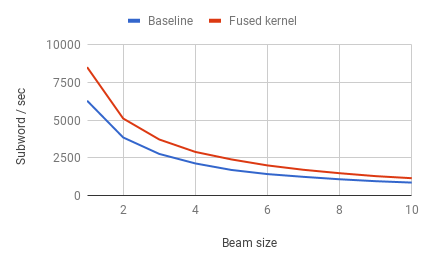
\includegraphics[scale=0.5]{beam-opensubtitles.png}} 
\end{tabular}
\caption{Speed using the fused kernel}
\label{fig:beam-opensubtitles}
\end{figure} 

\subsection{Top-up Batching}

After some experimentation, we decided to top-up the decoding batch only when it is at least half empty, rather than whenever a sentence has completed.

The top-up batching and maxi-batching have similar goals of maximizing efficiency when translating batches of different lengths. The top-up batching is of limited utility when used with maxi-batching but it increases translation speed by up to 12\% when used alone, Figure~\ref{fig:topup-opensubtitles}.

\begin{figure}
\centering
\begin{tabular}{cc}
{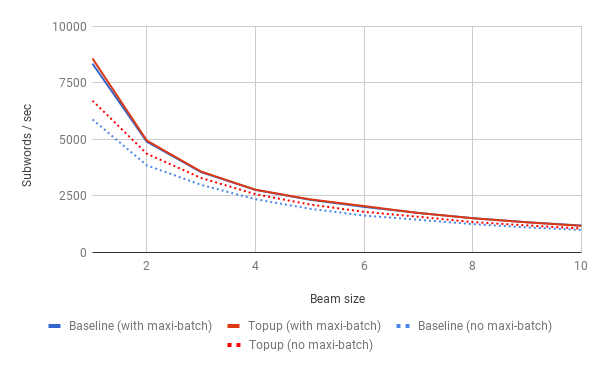
\includegraphics[scale=0.3]{topup-opensubtitles.png}} 
\end{tabular}
\caption{Speed using top-up batching}
\label{fig:topup-opensubtitles}
\end{figure} 

\subsection{Cummulative Results}

Using both the fused kernel and top-up batching to translate led to a cummalative speed improvement of up to 57\% when no maxi-batching is used, Figure~\ref{fig:cummulative-opensubtitles}. With maxi-batching, the speed was up to 41\% faster.

\begin{figure}
\centering
\begin{tabular}{cc}
{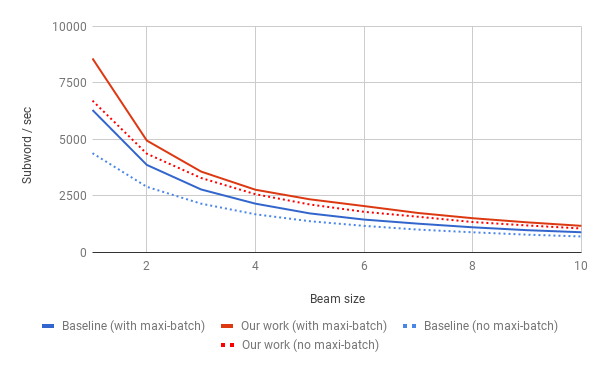
\includegraphics[scale=0.3]{cummulative-opensubtitles.png}} 
\end{tabular}
\caption{Cummulative results}
\label{fig:cummulative-opensubtitles}
\end{figure} 

%\section*{Acknowledgments}
%This work is sponsored by the Air Force Research Laboratory, prime contract FA8650-11-C-6160.  The views and conclusions contained in this document are those of the authors and should not be interpreted as representative of the official policies, either expressed or implied, of the Air Force Research Laboratory or the U.S. Government.

\bibliographystyle{apalike}
\bibliography{amta2016,mt,more}


\end{document}
\grid
